\subsection{Data Collection}
For the data collection, a barebones Android app was developed, which reads the triaxial accelerometer and gyroscope data at a constant rate of 50hz.
Additionally, timestamps and a unique device identifier were appended to each entry, along with an option to label recording sessions, all to simplify the processing pipeline and 
avoiding the need to manually label all the data afterwards.\\
Using this app, several activities were carried out and recorded, whilst trying to vary the conditions as much as possible, such as putting it in the left and right pockets and having it upside down or upright, aiming to diversify the data.  

\begin{figure}[htp]
    \centering
    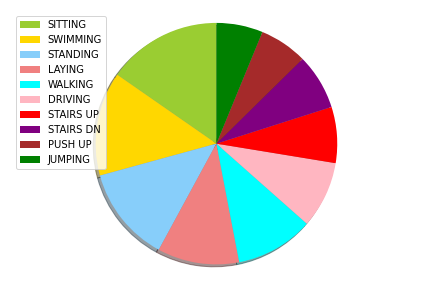
\includegraphics[width=.36\textwidth]{ethan_data_dist_pie}
    \caption{Our Data Distribution}
    \label{our_data_count_dist}
    \end{figure}

Figure \ref{our_data_count_dist} depicts the different amounts of data 
collected per activity. Unfortunately, there was a considerable difference in the amounts of data, where some activities such as jumping had much less data than other activities like walking. 
This can lead to the accuracy of classification of data to be misleading, since if for example the classifier is completely random, and it guesses 'walking', it is more likely to be right than if it randomly guesses 'jumping', 
and since there is more walking data, it may seem more accurate than it really is.

\subsection{Signal Processing}
The JSON data exported from the mobile application was then ready to be imported by a python preprocessor. As is, the data is not usable by the classifiers, not only does it contain a lot of noise, but a single entry gives very little information about what is happening.\\
Consequently, several steps were taken to maximise the usability and the potential for classification of the data, such as synchronisation of gyroscope and accelerometer signals, use of a sliding window to group data, signal filtering and feature extraction using several statistical measures.   

\subsection{Synchronisation}
Due to a limitation from the application, the gyroscope and accelerometer collections worked asynchronously, and thus the entries were likely not to be aligned properly (a few milliseconds of difference). And if the phone screen was turned off, data collection would stop and restart when the screen is turned on, which would cause a substantial gap within the data of a session.\\
A moving average of the differences was calculated over all the data. If the average difference is below 10ms, the values would be considered as forming part of the same timestamp, whilst if the average value was larger, an entry was removed from the accelerometer and gyroscope data, until the average restabilized. Thie eliminates most outliers, and if there are antired out of synch by a substantial margin, they are removed. This was considered quite harshly, as several techniques such as Fast Fourier transform rely on constant frequencies to provide desirable outputs. 
The first and last 2 seconds were also removed for each session, as time needs to be accounted for whilst the user puts the device in his/her pocket, which would provide inaccurate data. 


\subsection{Sliding Window}
As carried out in \cite{Noor2017} a sliding window of size 128 with a stride of 64 was adopted, which in simpler terms means grouping 128 entries (2.56 seconds of data) for each window, and overlap each window by 1.28 seconds.\\
This is one of the most crucial steps in data processing, as one single entry does not describe a whole lot about what a user is doing. Before any preprocessing, each entry simply has six values (two triaxial vectors), which are at a single point in time. When the sliding window is introduced, we group a window’s worth of entries into one, out of which we get a representation of what happens over a period (2.56 seconds in our case), where each window will represent 128 raw entries, containing 6 features (triaxial data) each. Which when feature mapped, summarizes features of this two-dimensional data frame, back into a one-dimensional entry, whilst still retaining the fact that an entry has now the added dimension of time.

\subsection{Signal Filtering}
A set of transformations were applied to each window of entries, which were used to filter and prepare the data for the feature extraction stage.

\subsubsection{20hz Butterworth Filter}
A low-pass Butterworth filter with a corner frequency of 20hz, which removes most of the noise, as most changes in the acceleration happened at much lower frequencies, and through this separation, the most relevant changes in acceleration were kept. In fact, according to \cite{Karantonis2006} most bodily movements are contained below 15Hz.

\subsubsection{0.3hz Butterworth Filter}
Another low pass Butterworth filter was applied with a corner frequency of 0.3hz, which filter separates gravitational acceleration from body acceleration, since changes in gravitational acceleration happen relatively slowly, a low corner frequency can distinguish and extract these changes as gravitational acceleration. 
\begin{figure}[htp]
    \centering
    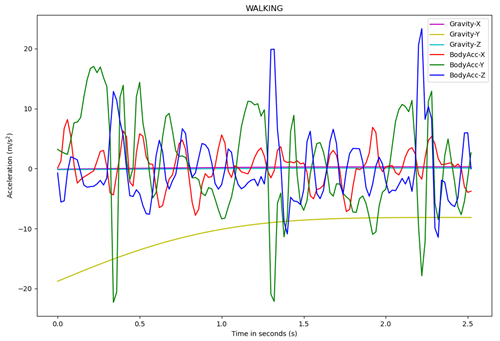
\includegraphics[width=.49\textwidth]{ethan_window_acc_plot}
    \caption{The Acceleration in a single window}
    \label{fig:figure_single_wind}
    \end{figure}

Figure \ref{fig:figure_single_wind} shows the 
different forces of acceleration experienced whilst the user was walking.
The Body forces show the filtered acceleration when separated from the gravitational acceleration. At idle, these forces should be zero. 
The strides of the user's walking may also be observed as fluctuations in the green line, quickly dropping when the wearer’s foot descends and hits the floor. 
The other three stable plots are the gravitational forces experienced, these should not change as much, as the gravitational force experienced does not fluctuate quickly. At idle the vector of these three forces should point 
downwards with a magnitude of \textasciitilde $9.81m/s^2$.

\subsubsection{The Jerk}
Jerk is defined as the change in acceleration and was calculated by differentiating the acceleration values by time: $\delta t = 1/50hz = 0.02s$. This gives a better idea of how drastically the accelerations change, such as when one is jogging and the leg where the phone is sitting stops sharply as it hits the ground.

\subsubsection{The Magnitude}
The magnitude is the measure of how much the values differ from zero. This comes useful when one simply needs an idea of the amount of force applied, without considering the effects of directionality.

\subsubsection{Fast Fourier Transform}
FFT enabled the calculation of frequency components based on the time-varying signals. When considering Human Activity, one can note that there is a lot of repetitive patterns, in which case transformations such as FFT are used to calculate the discrete Fourier transform, and give a
rich statistic for summarizing a window of these repetitive signals \cite{SousaLima2019}.

\subsection{Feature Extraction}
    Excluding the label for each activity, each session in the dataset contains 589 features. These features were extracted by applying a number of different statistical
    measures to the different extracted signals in each sliding window.

    Each signal has the statistical measures in \ref{fig:features_table1} applied to them.

    \begin{figure}[H]
        \centering
        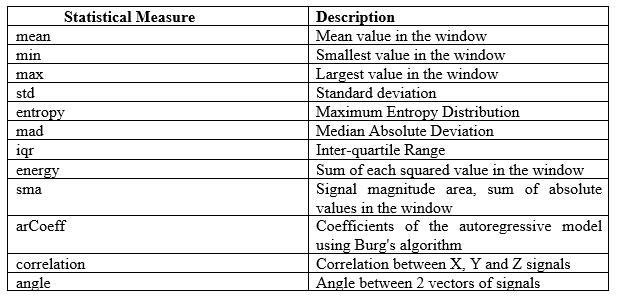
\includegraphics[scale=0.55]{jake_table_1}\hfill
        \caption{Statistical Measures}
    \label{fig:features_table1}
    \end{figure}

    The statistical measures in \ref{fig:features_table2} are applied only to FFT signals.

    \begin{figure}[H]
        \centering
        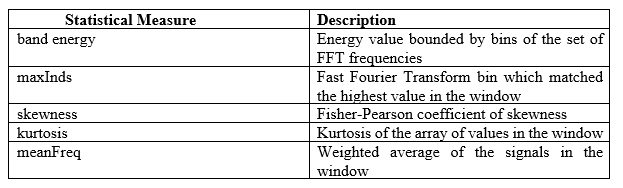
\includegraphics[scale=0.55]{jake_table_2}\hfill
        \caption{Statistical Measures}
    \label{fig:features_table2}
    \end{figure}

\subsection{Signal Processing}

\subsection{Support Vector Machine Classifier}
\subsubsection{Data Pre-Processing}
    Firstly, the training and testing datasets were converted to Pandas dataframes and the labels for each activity were separated into their own variables.
    Using a LabelEncoder, each activity label is converted into a numerical value.

\subsubsection{Comparing Different Classification models}
    In total, four different classic machine learning classifiers were used on the dataset developed by Anguita et al \cite{Anguita2012}. These classifiers are Gaussian Naïve Bayes,
    AdaBoost, Stochastic Gradient Descent and a Support Vector Machine. These were trained and tested using the respective datasets, and their accuracy,
    F-beta, precision and recall scores were recorded.

    \begin{table}[ht]
        \centering\scriptsize
        \begin{tabular}{|l|l|l|l|l|}
            \hline
            \textbf{Classifier} & \textbf{Accuracy} & \textbf{F-Beta}  & \textbf{Precision} & \textbf{Recall} \\ \hline
            Gaussian Naïve Bayes             & 0.7134           & 0.7252  & 0.7555 & 0.7134 \\ \hline
            AdaBoost            & 0.4065           & 0.2520 & 0.4289 & 0.4065 \\ \hline
            Stochastic Gradient Descent               & 0.9600           & 0.9603 & 0.9605 & 0.9600 \\ \hline
            Support Vector Machine            & 0.9668           & 0.9676 & 0.9682 & 0.9668 \\ \hline
        \end{tabular}
        \caption*{Table 3: Performance scores of each classifier}
    \end{table}

    As can be seen in Table 3, the Stochastic Gradient Descent classifier and the Support Vector Machine had the highest scores, with each result being over 0.96.
    However, the SVM's performance metrics had slightly higher results. Furthermore, the cost function in Stochastic Gradient Descent is based on a single set of samples
    in the training data and its positive results do not translate to accurate results in the testing phase. It is for this reason that the Support Vector Machine classifier
    was chosen to classify the UCI dataset \cite{Anguita2013} and, later on, the dataset built by ourselves.

\subsection{Classification}
    The RBF kernel is defined as the exponential function \(exp(-\gamma \lvert x-x' \rvert)^2\) \cite{Scholkopf2004}, where $x$ and $x’$ are two feature vectors, and $\gamma$ is the
    gamma parameter in the classifier. Gamma’s value is scale, meaning that the parameter is the reciprocal of the number of features multiplied with the variance of the input data.
    For this implementation, we opted for a One-Vs-All approach. A One-Vs-All approach divides the data points into just two classes: a certain activity and the other classes. Therefore records
    labelled as \emph{SITTING} are a single class, and the other activities are treated as having a single label.

\subsection{Convolutional Neural Networks}
The implementation described in this report is based on the architectures described by Cho et al. \cite{Cho2018}.
Unlike Cho et al. we did not implement a first stage dynamic-static split model and instead opted to split the labels manually.
The Pytorch library was used to implement the CNNs, and the sklearn library to evaluate the results.

\subsubsection{Data Split}
The train/valid/test split was an 80/20 train/test split, then 80/20 train/validation split for the UCI dataset, and a 90/10 train/test split, then 90/10 train/validation split for Our Dataset.

\subsubsection{Dataset Object}
To facilitate this dynamic/static split we defined a Python dictionary with each label having a number assigned to it, starting from 0.
The numbering needs to start from 0 as the output of neural networks implemented in Pytorch always start from 0.
Another requirement for implementing neural networks in Pytorch is to implement a custom Dataset object.
The function of this object is to read the data from a source and define its X, data and Y, labels counterparts.
The Pandas library was used at this stage due to its use of the numpy library and efficient data management.
It is important that the X component is in the shape: length(data.columns), 1, length(data.rows)).

The dataset object was initialised 3 times, for the Train, Validation and Testing data.

The pie charts included below show the training, validation and testing label distribution in order.

\begin{figure}[H]
\centering
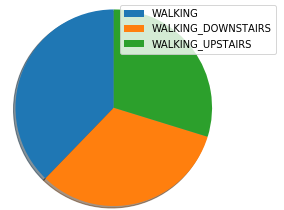
\includegraphics[width=.15\textwidth]{UCI_Dynamic_Training}\hfill
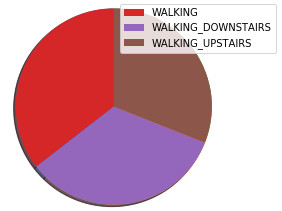
\includegraphics[width=.15\textwidth]{UCI_Dynamic_Validation}\hfill
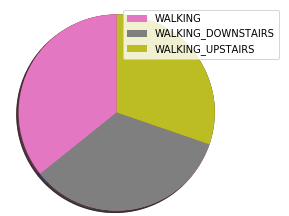
\includegraphics[width=.15\textwidth]{UCI_Dynamic_Testing}
\caption{UCI Dynamic Label Distribution}
\label{fig:UCI_Dynamic_Distribution}
\end{figure}

\begin{figure}[H]
\centering
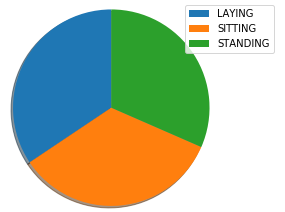
\includegraphics[width=.15\textwidth]{UCI_Static_Training}\hfill
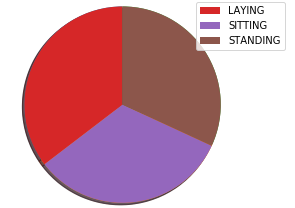
\includegraphics[width=.15\textwidth]{UCI_Static_Validation}\hfill
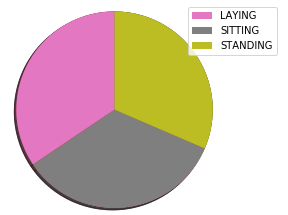
\includegraphics[width=.15\textwidth]{UCI_Static_Testing}
\caption{UCI Static Label Distribution}
\label{fig:UCI_Static_Distribution}
\end{figure}

\begin{figure}[H]
\centering
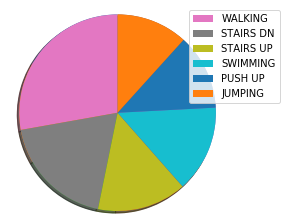
\includegraphics[width=.15\textwidth]{OD_Dynamic_Training}\hfill
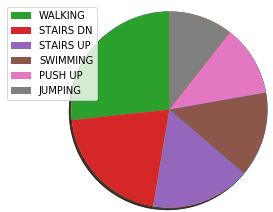
\includegraphics[width=.15\textwidth]{OD_Dynamic_Validation}\hfill
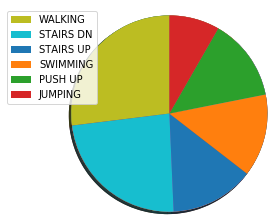
\includegraphics[width=.15\textwidth]{OD_Dynamic_Testing}
\caption{OD Dynamic Label Distribution}
\label{fig:OD_Dynamic_Distribution}
\end{figure}

\begin{figure}[H]
\centering
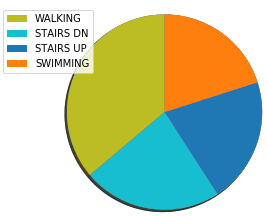
\includegraphics[width=.15\textwidth]{OD_Static_Training}\hfill
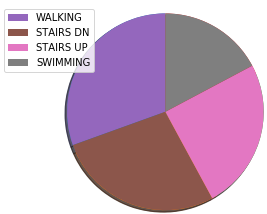
\includegraphics[width=.15\textwidth]{OD_Static_Validation}\hfill
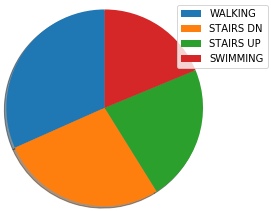
\includegraphics[width=.15\textwidth]{OD_Static_Testing}
\caption{OD Static Label Distribution}
\label{fig:OD_Static_Distribution}
\end{figure}

In development, it was noted that the data distribution of the dynamic activities in our dataset was unequal.
This was causing issues with the CNN's accuracy.
To combat this added functionality was added with the aim of increase the quality of the model's output.
In this project the number of rows for each eligible label was stored.
Using the functionality provided by the Pandas library, the index for each label was stored in a list linked to its respective label.
Using Python list slicing these lists where cut down to their lowest common length.
These indices where then converted into a new Pandas dataframe and this balanced dataset was used for the dynamic model.

\begin{figure}[H]
\centering
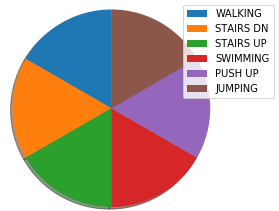
\includegraphics[width=.15\textwidth]{OD_Dynamic_Training_Balanced}\hfill
\caption{OD Dynamic Training Balanced Label Distribution}
\label{fig:Balanced_Train}
\end{figure}

Finally, the dataset objects are used to initialise a Dataloader object.
This object gives us the functionality of delivering batches as inputs to the models at training and testing.
It was found that a batch size of 32 worked best for the Static models, and a batch size of 64 worked best for the dynamic models.

\subsubsection{Model Creation}
The CNN models were implemented following the design of the below diagrams.
Every model used the Cross-Entropy as their loss function and the ADAM optimizer.
The learning rate for the UCI Dataset Models and Our Dataset Static model was set at 0.0005 and were trained for 10 epochs.
The learning rate for the Our Dataset Dynamic model was set at 0.00005 and were trained for 11 epochs.

\begin{figure}[H]
\centering
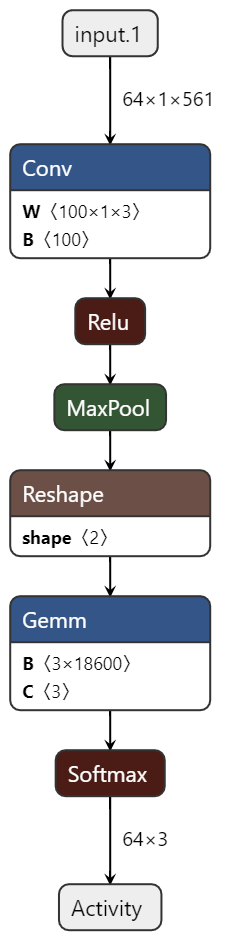
\includegraphics[width=.15\textwidth]{DCNN}\hfill
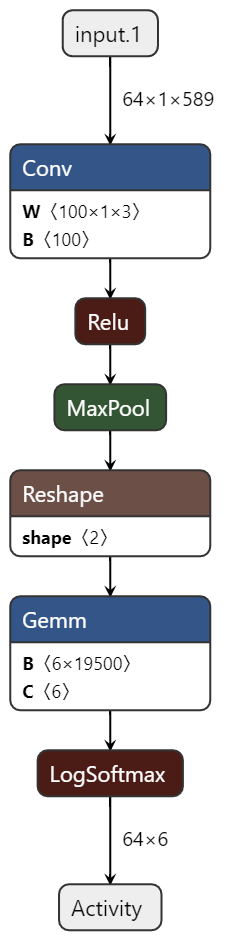
\includegraphics[width=.15\textwidth]{ODDCNN}\hfill
\caption{UCI(left) and OD(right) Dynamic Model Structure}
\label{fig:Dynamic_Models}
\end{figure}

\begin{figure}[H]
\centering
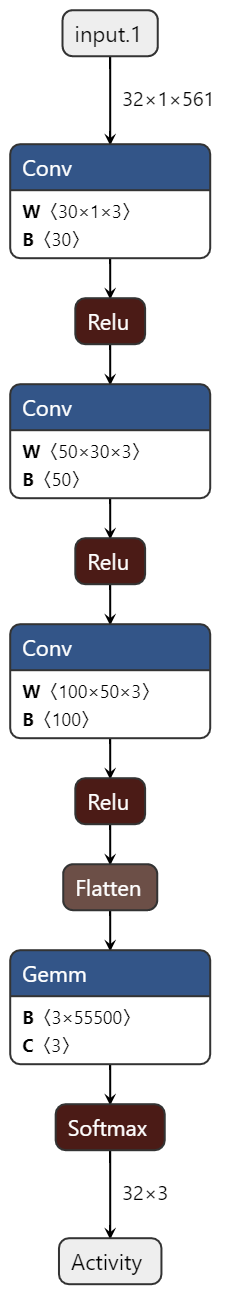
\includegraphics[width=.15\textwidth]{SCNN}\hfill
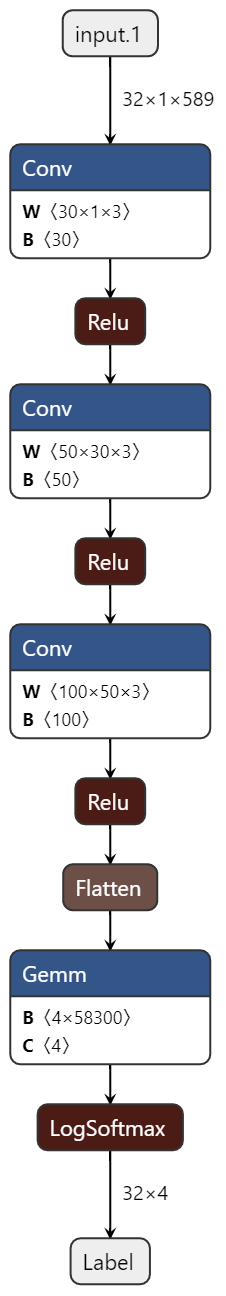
\includegraphics[width=.15\textwidth]{ODSCNN}\hfill
\caption{UCI(left) and OD(right) Static Model Structure}
\label{fig:Static_Models}
\end{figure}

As seen in figures \ref{fig:Static_Models} and \ref{fig:Dynamic_Models} the four models follow the a similar structure having a Convolutional layer that is then followed by a fully connected layer.
The OD models differentiate at the final activation function where it was found that the Softmax activation function was not activating properly.
Seeing this another activation function was used, the LogSoftmax function.
It is also worthwhile to note that the final layer fully connected layer is different since the UCI dataset and Our dataset have a different number of total features.
These models accept a tensor of the shape: (batchsize, 1, number\_of\_features).
The output of item in this batch is a number that corresponds to the encoded label.
Dropout is present at the fully connected layer, set to 50\% to combat overfitting.
Dropout is useful since it applies a 50\% chance of ignoring a neurons outputting, which forces the model to learn redundancy.